\documentclass[10 pt,usenames,dvipsnames, oneside]{article}
\usepackage{../../modelo-fracoes}
\graphicspath{{../../../Figuras/licao05/}}


\begin{document}

\begin{center}
  \begin{minipage}[l]{3cm}

\includegraphics[width=2cm]{../../../Figuras/logo}       
\end{minipage}\hfill
\begin{minipage}[r]{.8\textwidth}
 {\Large \scshape Atividade: }  
\end{minipage}
\end{center}
\vspace{.2cm}

\ifdefined\prof
%Caixa do Para o Professor
\begin{goals}
%Objetivos específicos
\begin{enumerate}
  \item     Entender o processo de determinação de um denominador comum entre duas frações com base na ideia de subdivisão da unidade da qual ambas sejam múltiplas inteiras, obtida a partir de um processo geométrico;
  \item     Determinar a soma e a diferença de duas frações a partir dessa subdivisão da unidade.
\end{enumerate}

\tcblower

%Orientações e sugestões
\begin{itemize}
  \item      Diferentemente da atividade anterior, nesta atividade a subdivisão da unidade já é dada, e sua determinação não é pedida ao aluno, o que voltará a ser objetivo das próximas atividades.
  \item      O item a) visa especificamente à identificação geométrica de subdivisão da unidade que será empregada para efetuar as operações. Espera-se     $\frac{1}{16}$     como resposta.
  \item     No item b), procura-se resgatar as atividades sobre frações equivalentes realizadas na lição 4. Observe que aqui há um processo de recontagem a partir da subdivisão ``pedaço de chocolate''. Aqui a fração equivalente indica a recontagem da fração $\frac{1}{2}$ a partir da subdivisão $\frac{1}{16}$.
  \item  No item c), procure destacar a interpretação de adição como ``juntar''. Pretende-se que o professor tenha a possibilidade de sistematizar a adição, tendo como apoio a resposta dos alunos dadas a partir de observações visuais. Isto é, o estudante pode dizer que, juntos, Alice e Miguel comeram 11 pedaços e depois identificá-los como $\frac{11}{16}$ da barra de chocolate. A discussão deve ser encaminhada a partir da determinação de frações equivalentes desenvolvida no item anterior (e {\bf sem} o uso do conceito de MMC). O objetivo é que o professor aproveite as soluções intuitivas dos alunos para apresentar, de forma mais sistematizada, a adição por uso de fração equivalentes, obtidas na busca de uma subdivisão comum:
$$\frac{1}{2} + \frac{3}{16} = \frac{8}{16} + \frac{3}{16} = \frac{11}{16}.$$
  \item  O item d) deve ser encaminhado de forma análoga ao anterior. Especificamente, deve-se retomar a ideia de que $1 = \frac{n}{n}$, discutida na lição anterior, daí apresentar $$1 - \frac{11}{16} =  \frac{16}{16} - \frac{11}{16} = \frac{5}{16}.$$
\end{itemize}
\end{goals}

\bigskip
\clearpage
\begin{center}
{\large \scshape Atividade}
\end{center}
\fi

Uma barra de chocolate é vendida com as marcações mostradas na figura abaixo.

 \begin{center}
 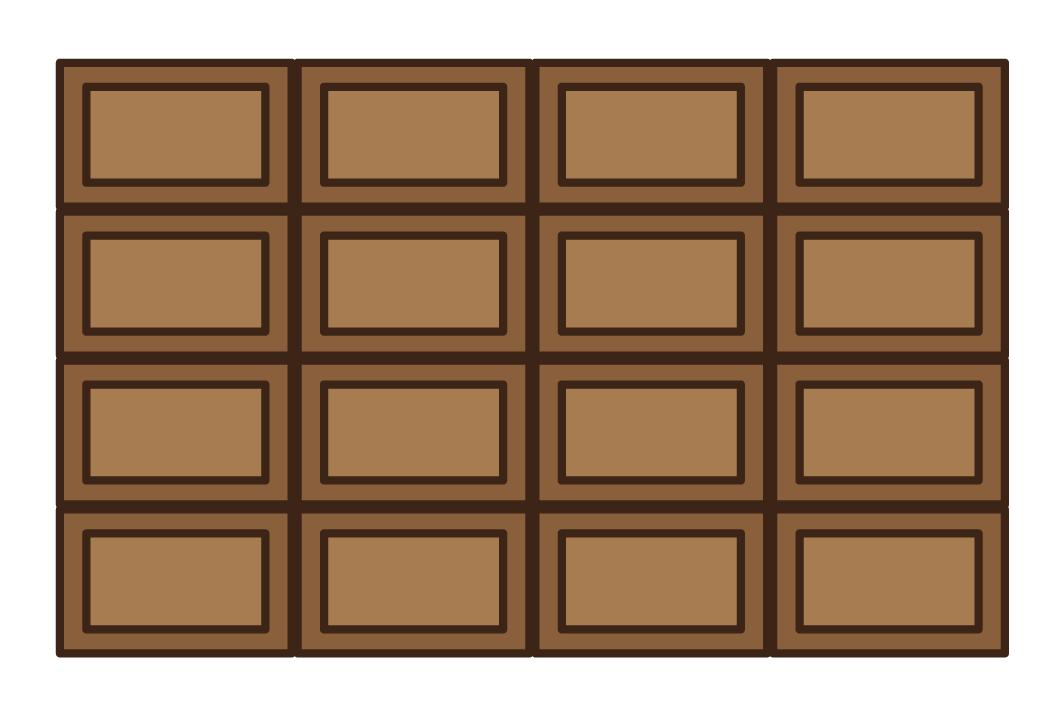
\includegraphics[width=150pt, keepaspectratio]{ativ3_fig01.png}
 \end{center}


Alice comeu a metade dessa barra de chocolate (em bege), quebrou o restante da barra em pedaços, seguindo as marcações e comeu 3 desses pedaços (em azul).

\begin{center}
\begin{tikzpicture}[x=1.0cm,y=1.0cm, scale=.7]
\fill[fill=light] (-1.,5.) -- (-1.,1.) -- (3.,1.) -- (3.,5.) -- cycle;
\fill[fill=common] (3.,5.) -- (5.,5.) -- (5.,3.) -- (3.,3.) -- cycle;
\fill[fill=common] (5.,5.) -- (7.,5.) -- (7.,4.) -- (5.,4.02) -- cycle;
\draw  (-1.,5.)-- (-1.,1.);
\draw  (-1.,1.)-- (3.,1.);
\draw  (3.,1.)-- (7.,1.);
\draw  (7.,1.)-- (7.,5.);
\draw  (7.,5.)-- (-1.,5.);
\draw  (3.,5.)-- (3.,3.);
\draw  (5.,5.)-- (5.,1.);
\draw  (-1.,3.)-- (7.,3.);
\draw  (-1.,2.)-- (7.,2.);
\draw  (1.,5.)-- (1.,1.);
\draw  (-1.,4.)-- (7.,4.);
\draw  (3.,3.)-- (3.,1.);
\end{tikzpicture}
\end{center}

Se considerarmos a barra de chocolate como a unidade, indicamos que as quantidades comidas são: $\frac{1}{2}$ por Alice e $\frac{3}{16}$ por Miguel.
Os pedaços da barra (quebrados por Miguel de acordo com as marcações na barra) correspondem a uma subdivisão dessa unidade.
Observe que ambas as frações da barra de chocolate comidas por Alice e Miguel podem ser obtidas a partir dessa subdivisão: Miguel comeu 3 pedaços e a quantidade comida por Alice corresponde a 8 pedaços.
\begin{enumerate}
\item Um pedaço corresponde a que fração da barra de chocolate?
\item Complete a parte em branco (numerador) para indicar a fração da barra de chocolate que Alice comeu.
$$\frac{1}{2} = \frac{\text{\Large $\square$} }{16}$$
\item Que fração da barra de chocolate foi comida por Alice e por Miguel, juntos?
\item  Que fração da barra de chocolate não foi comida?
\end{enumerate}

\ifdefined\prof
\begin{solucao}

\begin{enumerate}
     \item $\frac{1}{16}$.
     \item $\frac{1}{2}=\frac{8}{16}$, pois a fração equivalente a $\frac{1}{2}$ com denominador 16 é $\frac{8}{16}$.
     \item Observando as quantidades comidas por Alice e Miguel, a partir de um mesmo denominador, temos $\frac{1}{2}+\frac{3}{16} = \frac{8}{16} + \frac{3}{16} = \frac{11}{16}$.
     \item Recordemos que a barra de chocolate é a unidade de medida, então essa quantidade será entendida como 1 inteiro. Assim a quantidade restante será dada por $\frac{5}{16}$, pois $1 - \frac{11}{16} = \frac{16}{16} - \frac{11}{16} = \frac{5}{16}$.
\end{enumerate}

\end{solucao}
\fi

\end{document}